\chapter{Results}
\label{chap:results}

The first experiment is devoted to answer RQ1. We present a comparison between shallow and deep models. Table~\ref{tab:res1} shows AUC numbers for predictions performed using information acquired within the first 48 hours after the patient admission. Predictions performed by the baseline models were simply separated according to the ICU domain in which the corresponding patient was admitted, so that we can report AUC numbers for each ICU domain. On the other hand, the CNN$-$LSTM model employs domain adaptation, and thus is composed of four sub-models that are specific to each of the four domain ICUs. Clearly, domain adaptation improves the accuracy of our models and consistently outperform all baselines considered in this work. Overall, our model shows an AUC number of 0.818, which is considered to provide excellent clinical utility in the field of mortality prediction~\citep{revisited}.

\setlength{\tabcolsep}{3.5pt}
\renewcommand{\arraystretch}{1.1}
\begin{table}[htb]
\caption{AUC numbers for shallow and deep models. Numbers in bold indicate the best models for each ICU domain.}
\label{tab:res1}
\begin{center}
\begin{tabular}{lrrrr}
\hline
Model   & Cardiac & Coronary & Medical & Surgical\\ \hline
AdaBoost    & 0.572 & 0.551 & 0.510 & 0.531\\
SVM         & 0.627 & 0.572 & 0.503 & 0.532\\
LR          & 0.629 & 0.601 & 0.510 & 0.517\\
LDA         & 0.632 & 0.602 & 0.516 & 0.513\\
RF          & 0.610 & 0.578 & 0.587 & 0.623\\
QDA         & 0.689 & 0.668 & 0.567 & 0.610\\
\citep{kdd} & 0.853 & 0.802 & 0.760 & 0.785\\
CNN$-$LSTM  & \textbf{0.876} & \textbf{0.833} & \textbf{0.782} & \textbf{0.807}\\
\hline
\end{tabular}
\end{center}
%\end{table}
%\setlength{\tabcolsep}{6pt}
%\renewcommand{\arraystretch}{1}

\setlength{\tabcolsep}{4.4pt}   
\renewcommand{\arraystretch}{1.1}
%\begin{table}[htb]
\caption{AUC numbers for different feature transference approaches. Numbers in bold indicate the best transference approach for each target ICU domain.}
\label{tab:res2}
\begin{center}
\begin{tabular}{lllllll}
\hline
Target   & TT    & A1    & A2    & A3    & A4    & A5   \\\hline
Cardiac   & 0.821 & \textbf{0.876} & 0.863 & 0.864  & 0.805 & 0.814\\
Coronary  & 0.769 & \textbf{0.833} & 0.812 & 0.807  & 0.793 & 0.784\\
Medical   & 0.722 & 0.749          & 0.758  & \textbf{0.782} & 0.738 & 0.741\\
Surgical  & 0.727 & 0.802          & \textbf{0.807} & 0.798  & 0.756 & 0.756\\\cline{2-7}
Overall	  & 0.760 & \textbf{0.815}          & \textbf{0.811} & \textbf{0.813}  & 0.773   & 0.774\\\cline{2-7}
\hline
\end{tabular}
\end{center}
\end{table}
\setlength{\tabcolsep}{6.0pt}
\renewcommand{\arraystretch}{1}

The second experiment is concerned with RQ2. We present a comparison between the TT model and models learned following our five feature transference approaches. Table~\ref{tab:res2} shows AUC numbers for predictions performed using information acquired within the first 48 hours after the patient admission. Feature transference is never detrimental when compared with the TT model and they provide substantial gains that are up to 6.7\% (Cardiac), 8.3\% (Coronary), 8.3\% (Medical), and 11.0\% (Surgical). These gains seem to be related to the mortality rate associated with each target ICU domain $-$ gains are higher for domains with higher mortality rates.
%The exception occurs with the Medical ICU, which in turn is the largest domain, and therefore less prone to suffer from overfitting. 

\begin{figure}[htb]
\begin{center}
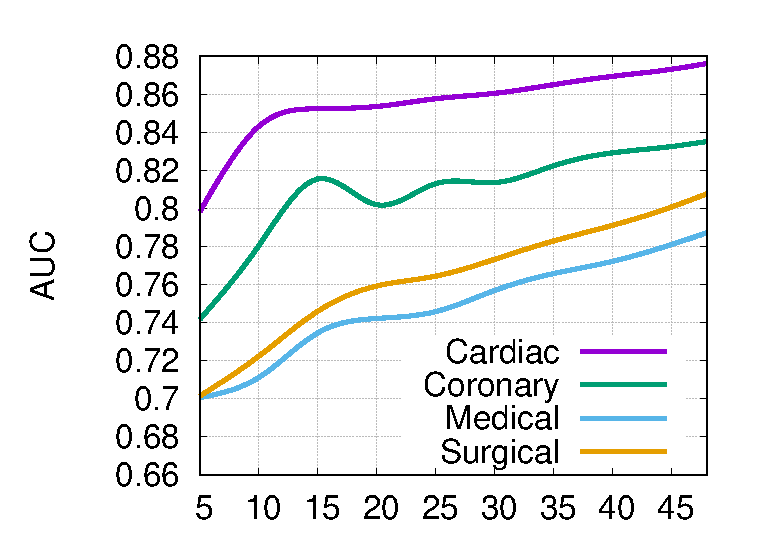
\includegraphics[width=0.82\linewidth]{figs/auc_time3}
\end{center}
\caption{(Color online) CNN$-$LSTM AUC numbers for predictions performed using information within the first $y$ hours after the patient admission ($5\le y\le48$).}
\label{fig:time1}
%\end{figure}
%\begin{figure}
\begin{center}
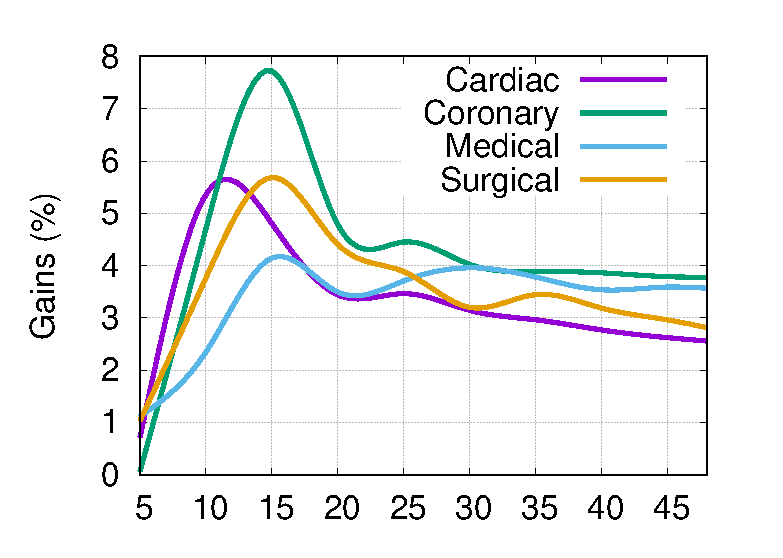
\includegraphics[width=0.82\linewidth]{figs/auc_time4}
\end{center}
\caption{(Color online) Gains over~\citep{kdd} at different prediction times ($5\le y\le48$).}
\label{fig:time2}
\end{figure}

Finally, we can see from Table~\ref{tab:res2} that the best transference approach varies depending on the target ICU domain. Randomly initializing the weights for fine-tuning does not show to be the best approach, as A4 and A5 were not the best performers for any target ICU domain. It seems that specific temporal patterns play an important role for mortality prediction in the Surgical domain, as A2 was the best transference approach for this domain. For the Medical domain, A3 was the best transference approach, suggesting that spatial and temporal features learned from other domains are already effetive. For the Cardiac and Coronary domains, A1 was the best transference approach, which indicates that specific spatial-temporal features are very important in these domains.

The next set of experiments is devoted to answer RQ3. Figure~\ref{fig:time1} shows AUC numbers obtained with predictions performed using information acquired within the first $y$ hours after the patient admission. As expected, accuracy increases as more information is acquired. From the first 5 to 20 hours, the slopes associated with Cardiac and Coronary domains increase much faster than the slopes associated with Medical and Surgical domains. 

Figure~\ref{fig:time2} shows the gains obtained when compared with the work by~\citet{kdd} at different prediction times. The early predictions performed by the CNN$-$LSTM archtecture are much more accurate than the early predictions performed by~\citet{kdd}, particularly in the first hours after the admission. The 10$-$20 hours period concentrates the more impressive gains, which vary from 4\% (Medical) to almost 8\% (Coronary).

\begin{figure*}[h!]
	\begin{center}
		\hspace{-0.3in}
		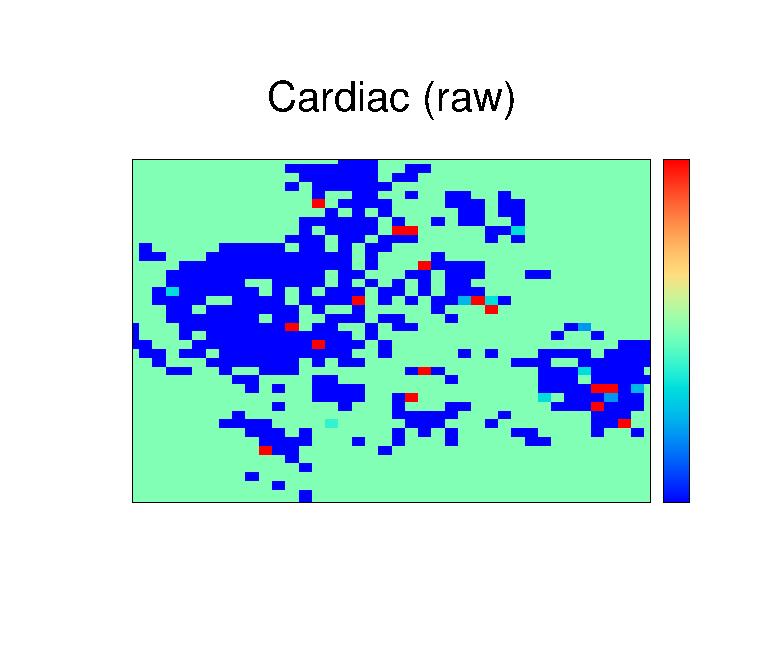
\includegraphics[width=0.305\linewidth]{figs/raw_cardiac}
		\hspace{-0.5in}
		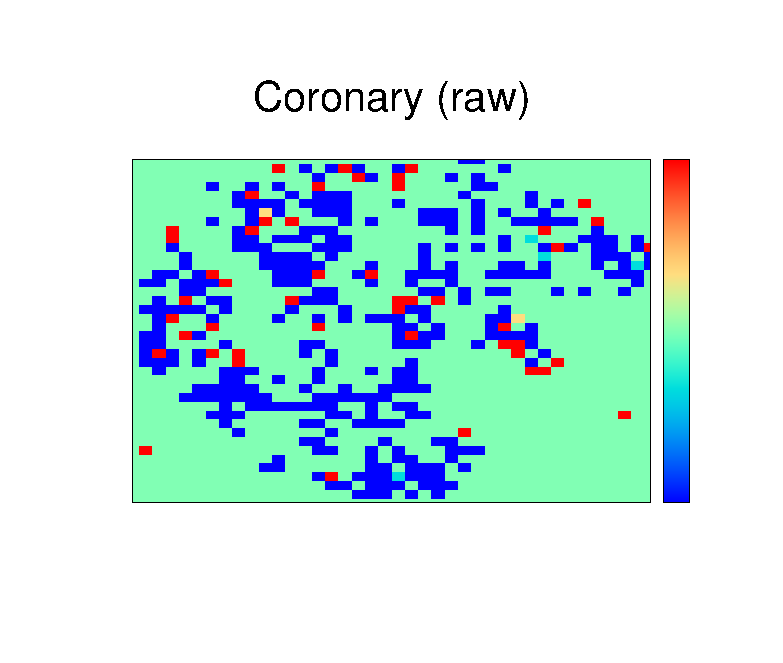
\includegraphics[width=0.305\linewidth]{figs/raw_coronary}
		\hspace{-0.5in}
		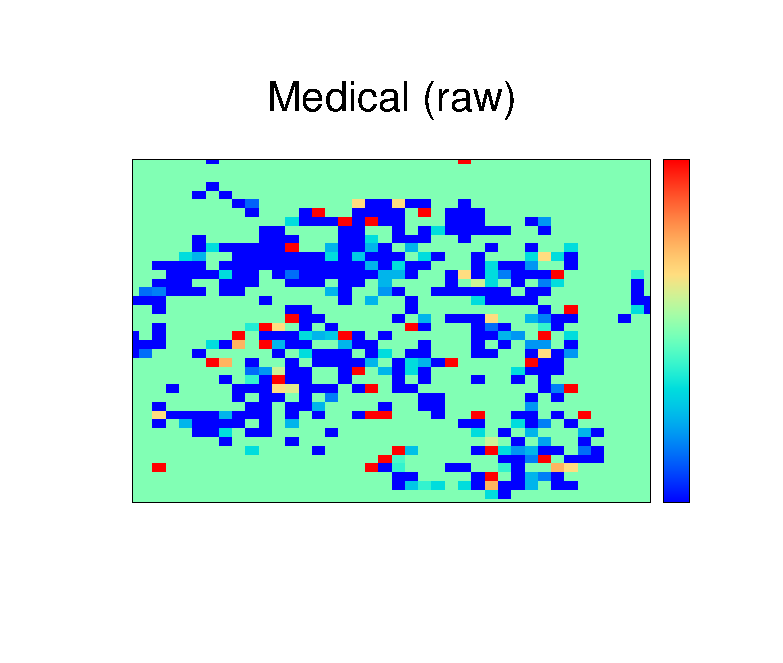
\includegraphics[width=0.305\linewidth]{figs/raw_medical}
		\hspace{-0.5in}
		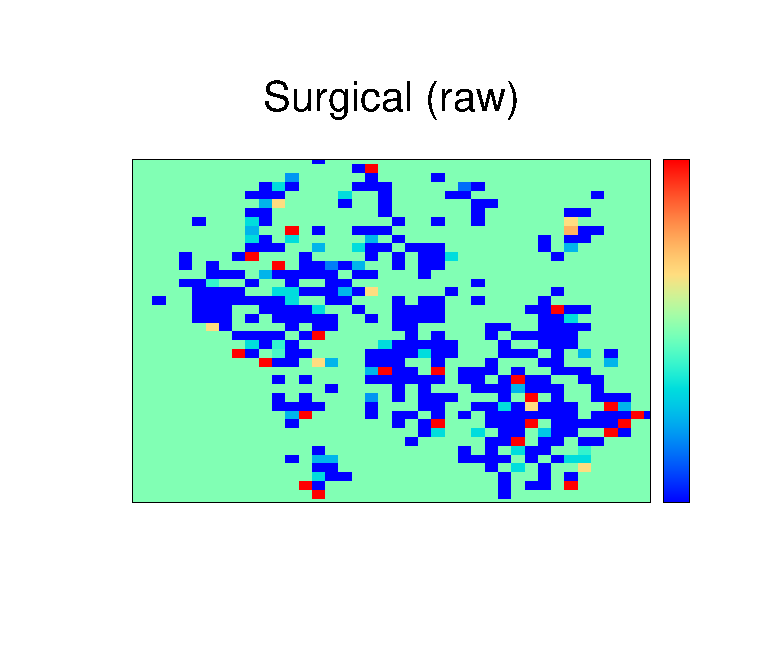
\includegraphics[width=0.305\linewidth]{figs/raw_surgical}\\
		\vspace{-0.4in}
		\hspace{-0.3in}
		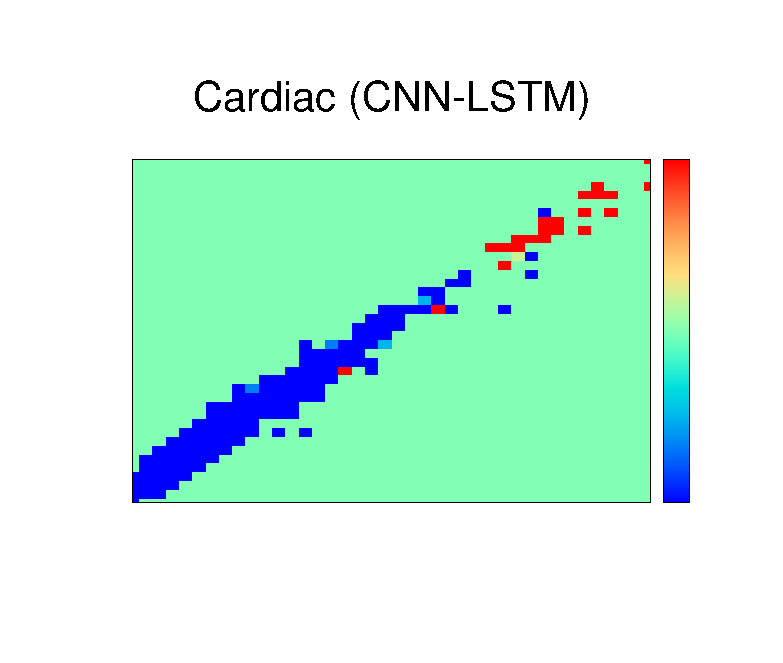
\includegraphics[width=0.305\linewidth]{figs/cardiac}
		\hspace{-0.5in}
		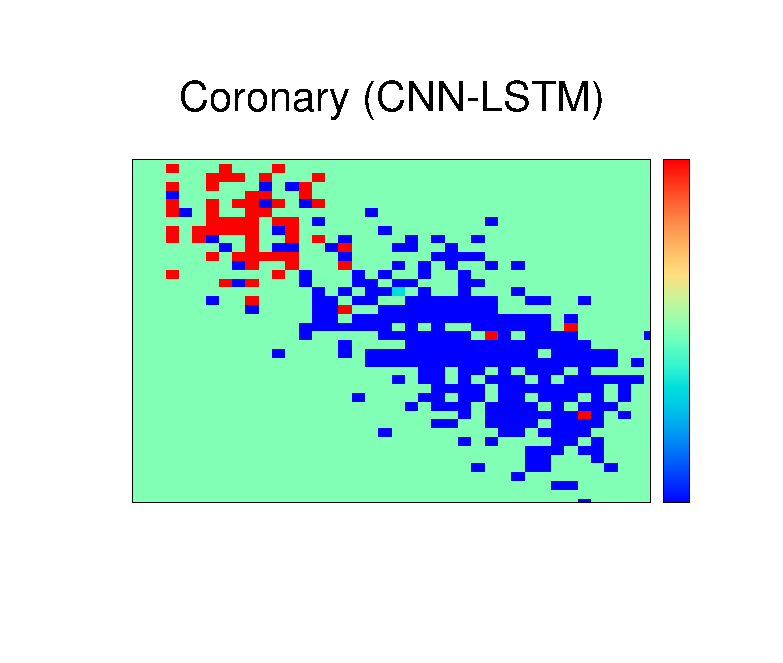
\includegraphics[width=0.305\linewidth]{figs/coronary}
		\hspace{-0.5in}
		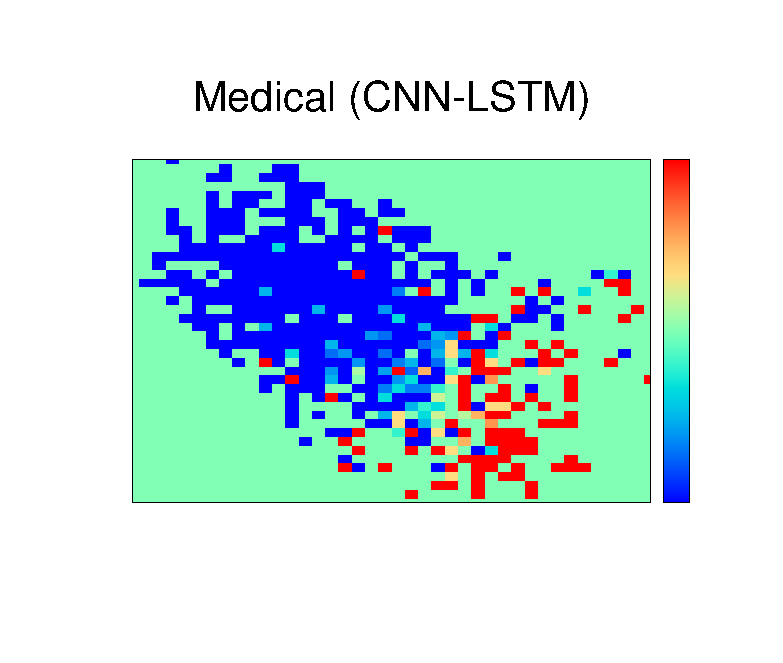
\includegraphics[width=0.305\linewidth]{figs/medical}
		\hspace{-0.5in}
		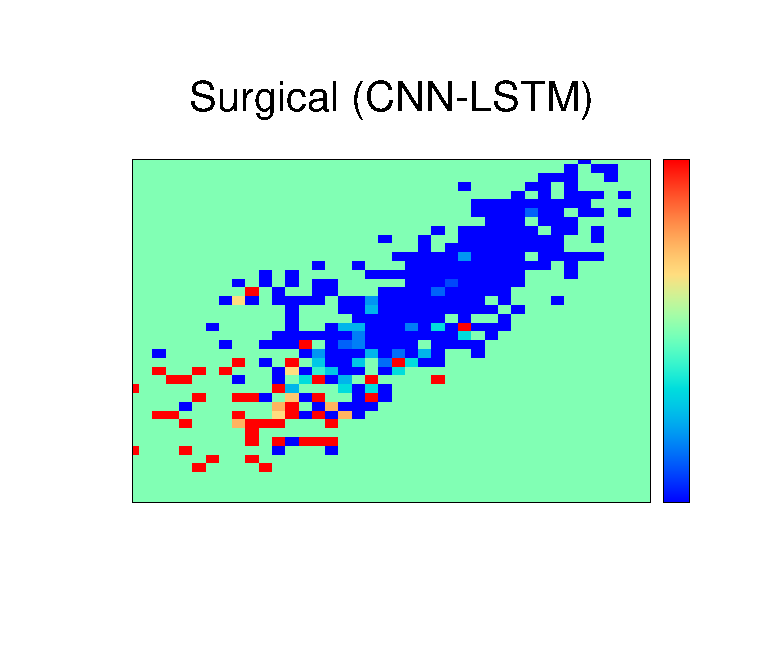
\includegraphics[width=0.305\linewidth]{figs/surgical}
		\vspace{-0.4in}
	\end{center}
	\caption{(Color online) Mortality risk space for different ICU domains. Regions in red are risky.}
	\label{fig:space}
	\begin{center}
		\hspace{-0.375in}
		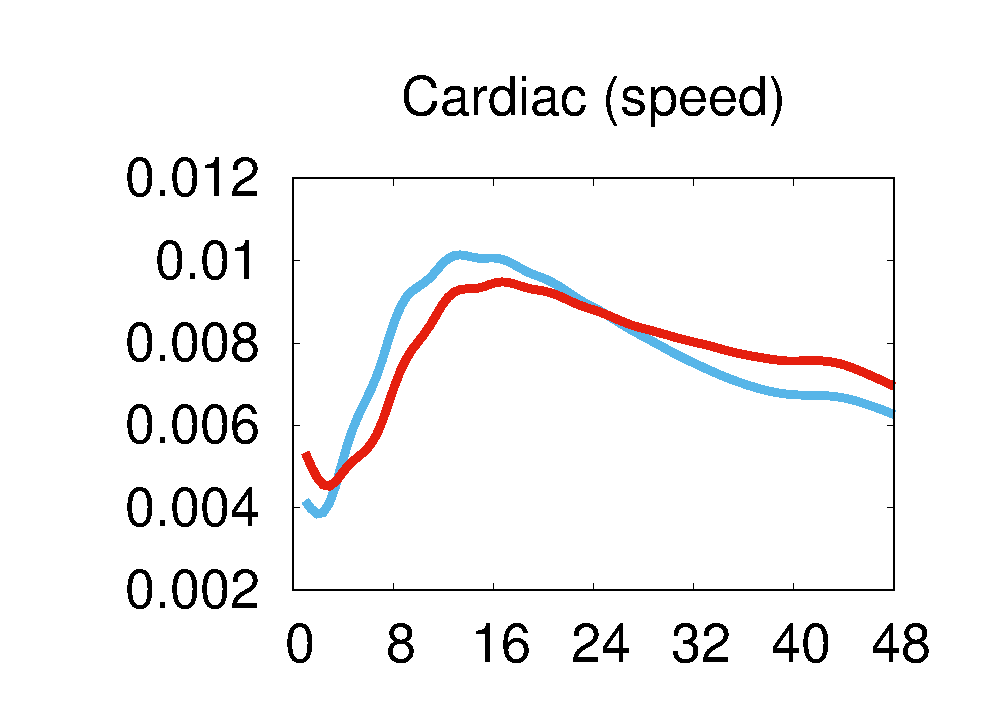
\includegraphics[width=0.295\linewidth]{figs/dynamics_speed_icu1}
		\hspace{-0.375in}
		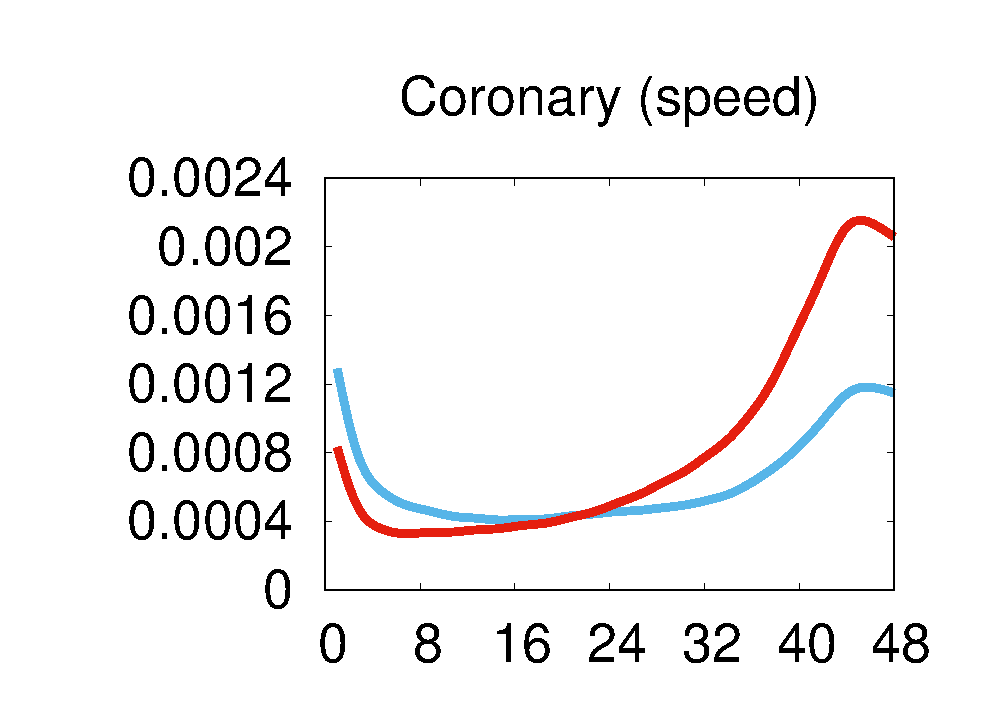
\includegraphics[width=0.295\linewidth]{figs/dynamics_speed_icu2}
		\hspace{-0.375in}
		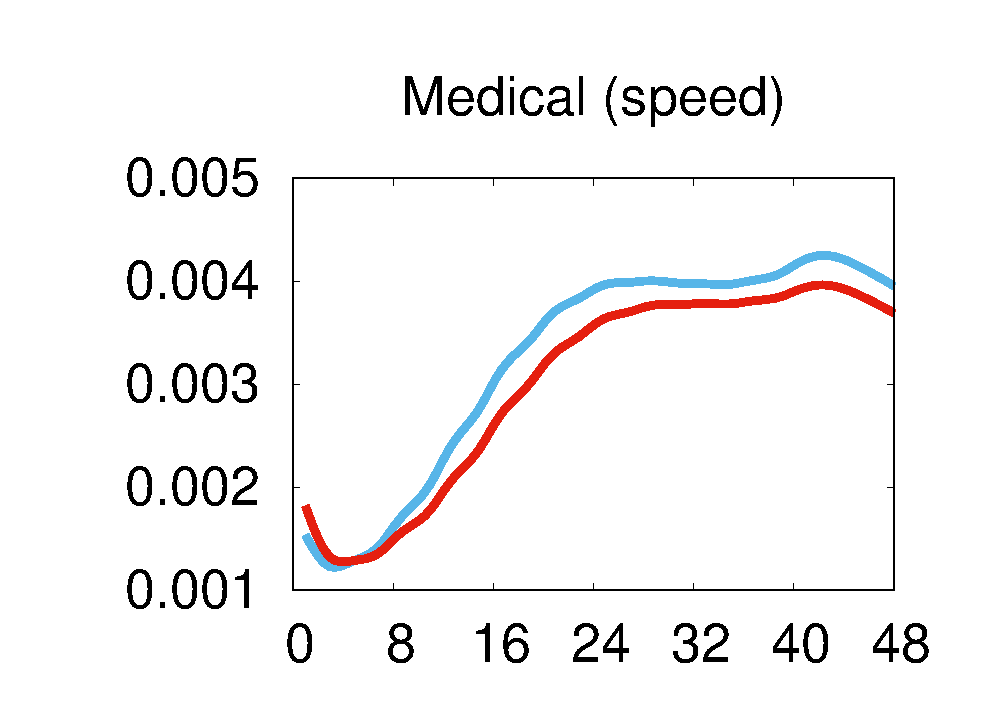
\includegraphics[width=0.295\linewidth]{figs/dynamics_speed_icu3}
		\hspace{-0.375in}
		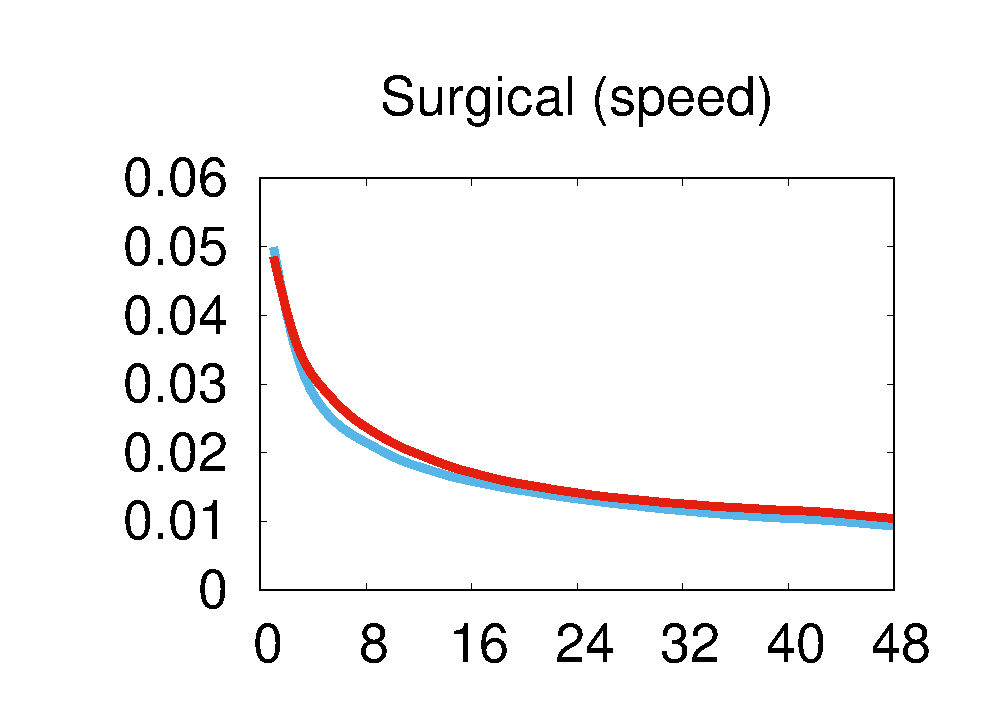
\includegraphics[width=0.295\linewidth]{figs/dynamics_speed_icu4}
		
		%\hspace{-0.375in}
		%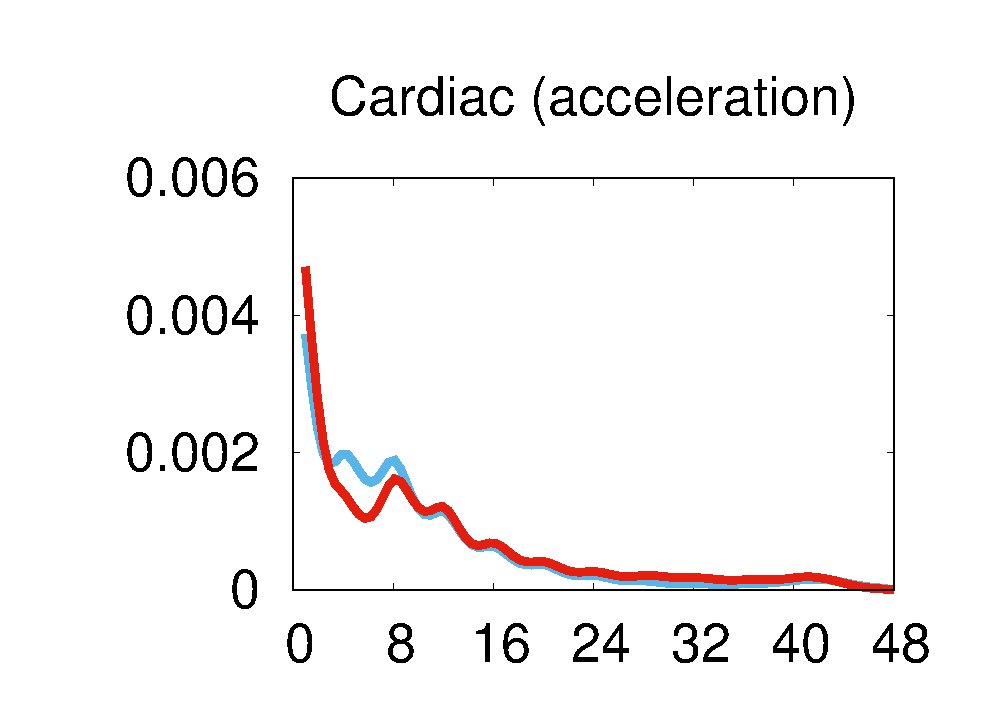
\includegraphics[width=0.295\linewidth]{figs/dynamics_acc_icu1}
		%\hspace{-0.375in}
		%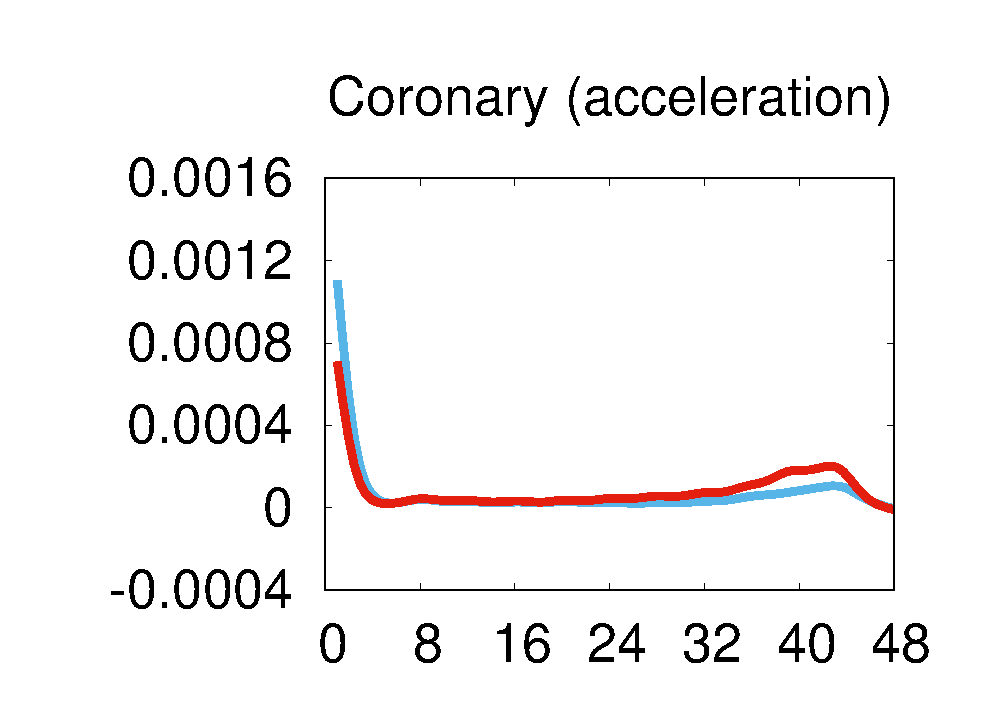
\includegraphics[width=0.295\linewidth]{figs/dynamics_acc_icu2}
		%\hspace{-0.375in}
		%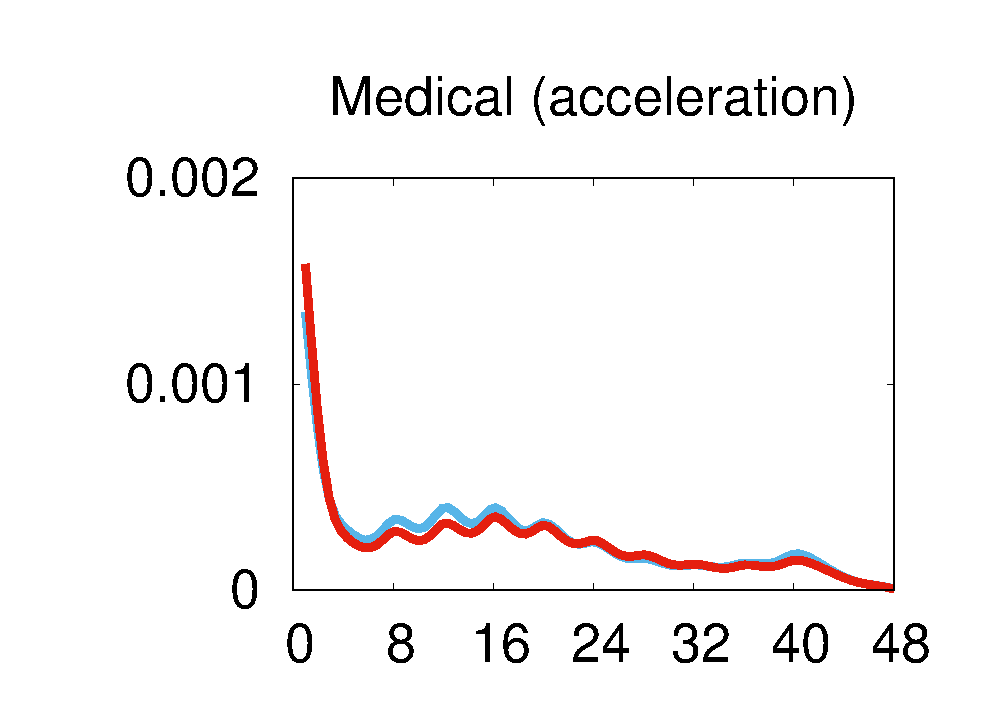
\includegraphics[width=0.295\linewidth]{figs/dynamics_acc_icu3}
		%\hspace{-0.375in}
		%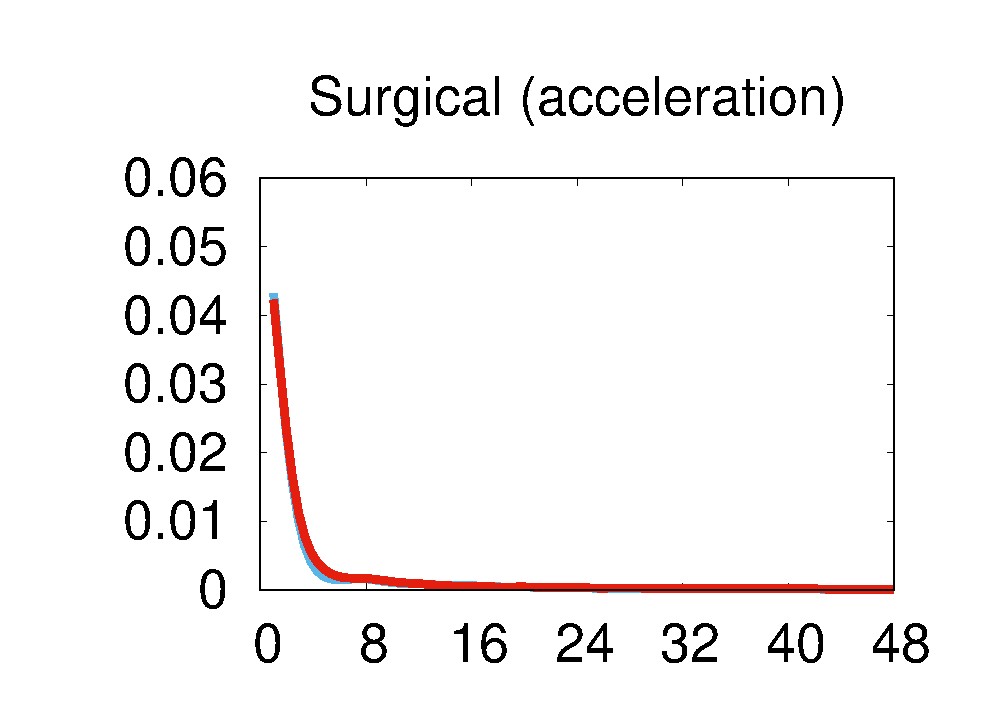
\includegraphics[width=0.295\linewidth]{figs/dynamics_acc_icu4}
		
		\hspace{-0.375in}
		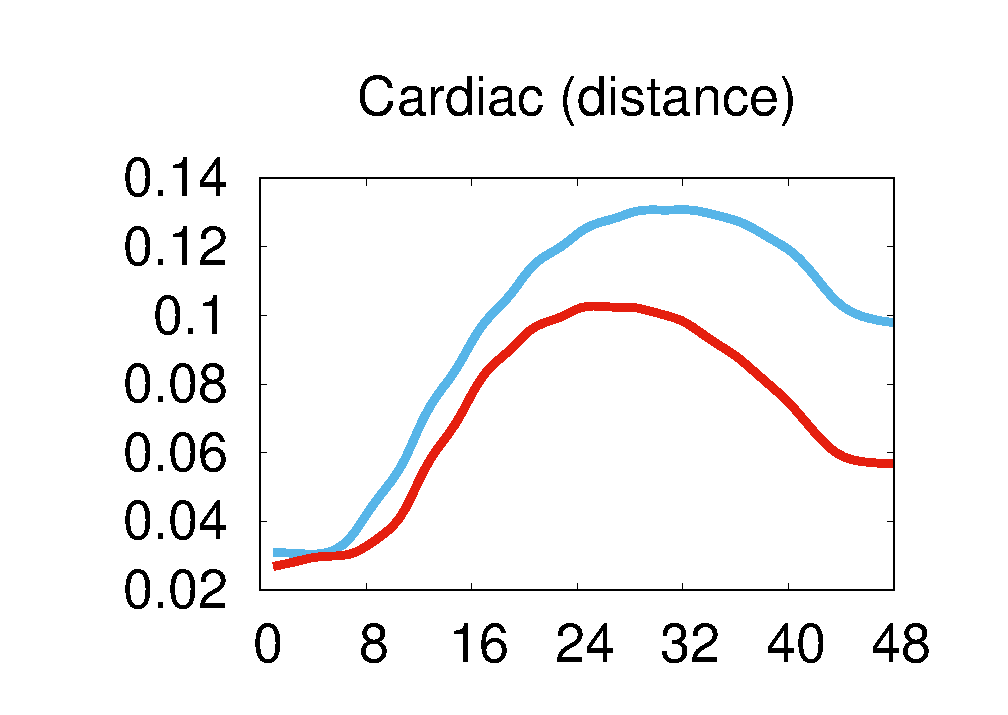
\includegraphics[width=0.295\linewidth]{figs/dynamics_dist_icu1}
		\hspace{-0.375in}
		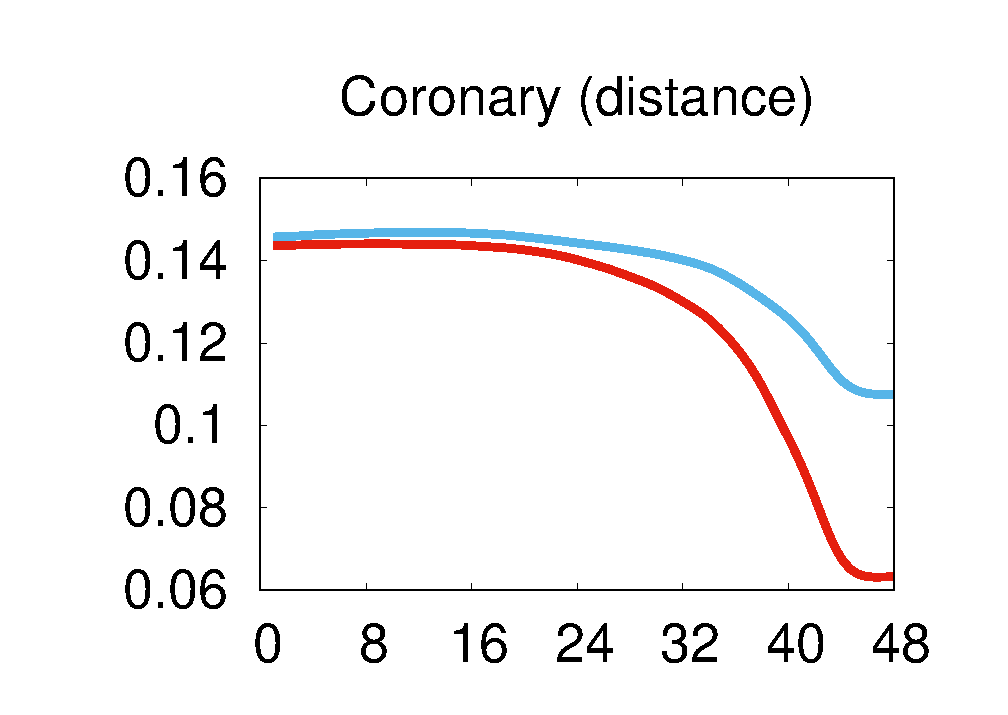
\includegraphics[width=0.295\linewidth]{figs/dynamics_dist_icu2}
		\hspace{-0.375in}
		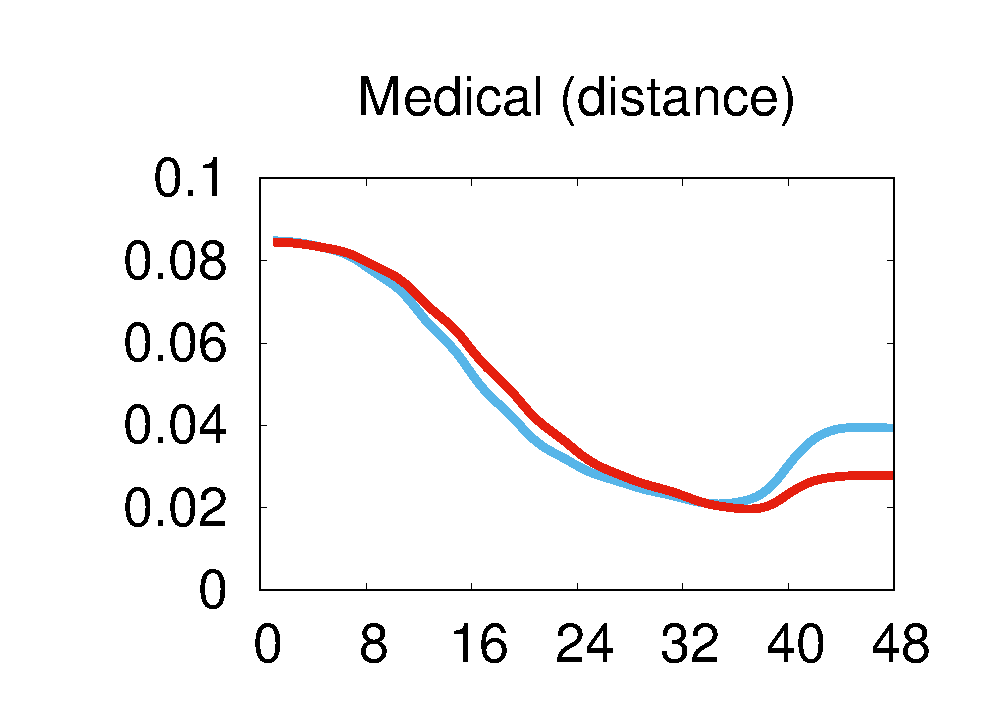
\includegraphics[width=0.295\linewidth]{figs/dynamics_dist_icu3}
		\hspace{-0.375in}
		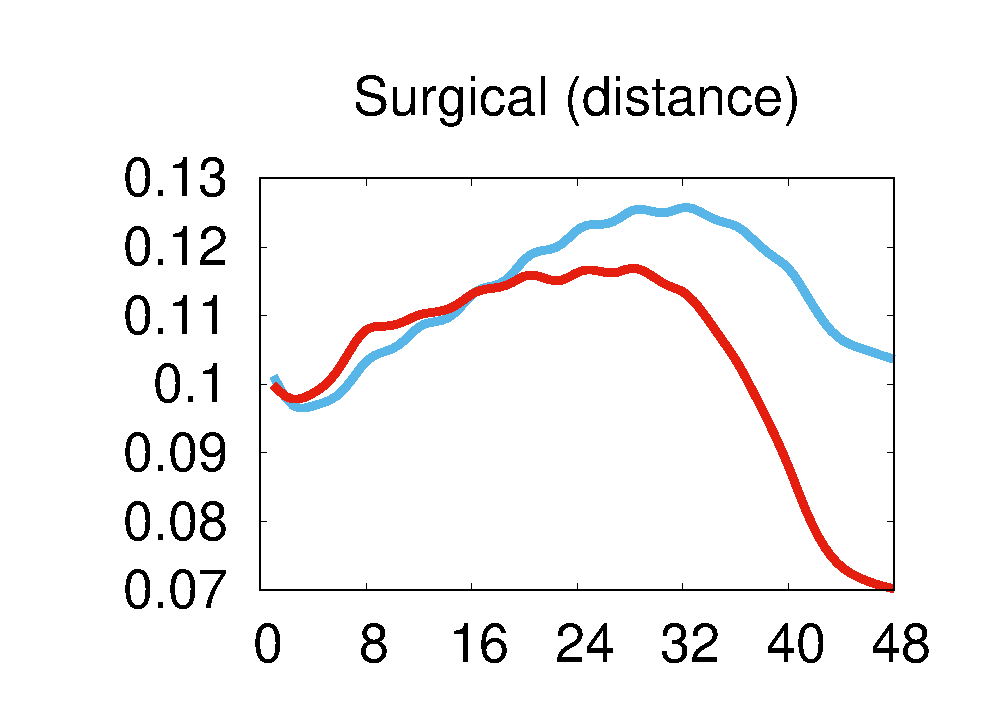
\includegraphics[width=0.295\linewidth]{figs/dynamics_dist_icu4}
	\end{center}
	\vspace{-0.134in}
	\caption{(Color online) Dynamics of 48-hour trajectories in different ICU domains. Red curves are computed from trajectories associated with patients that have died. Blue curves are computed from trajectories associated with patients that survived.}
	\label{fig:dynamics}
\end{figure*}

The last set of experiments is concerned with RQ4, i.e., to assess how meaningful are the mortality risk spaces. Figure~\ref{fig:space} shows risk spaces for each ICU domain. These spaces are obtained by gathering patient trajectories, that is, the coordinates (i.e., CNN$-$LSTM representations) along with the predicted outcome at each time. Risk spaces can also be obtained from raw data and, in this case, the coordinates are simply the entire feature-vector. Risk spaces created from CNN$-$LSTM representations are much more meaningful than the corresponding spaces obtained from raw data.

Time is also encoded in the risk spaces, and thus we can exploit dynamics, such as the proximity to mortality risky regions or the speed in which the patient condition changes. Figure~\ref{fig:dynamics} shows such dynamics in mortality risk spaces obtained from CNN$-$LSTM representations. Dynamics associated with the mortality risk space for the Cardiac and Coronary ICU domains, for instance, are highly discriminative since red and blue curves are separated in the first hours after the patient admission. This may explain the high AUC numbers obtained in these domains. Patients show distinct dynamics, depending on the ICU domain. Patients admitted to the Cardiac and Surgical units, for instance, move much faster than patients admitted to the Coronary and Medical units. Also, the speed increases over time for patients admitted to the Coronary and Medical units.